%%%%%%%%%%%%%%%%%%%%%%%%%%%%%%%%%%%%%%%%%%%%%%%%%%%%%%%%%%%%%%%%%%%%%%%%%%%%%%%%%%
\begin{frame}[fragile]\frametitle{}
\begin{center}
{\Large Concepts}
\end{center}
\end{frame}

%%%%%%%%%%%%%%%%%%%%%%%%%%%%%%%%%%%%%%%%%%%%%%%%%%%%%%%%%%%%%%%%%%%%%%%%%%%%%%%%%%
\begin{frame}[fragile]\frametitle{}
\begin{center}
{\Large Image Manifold}
\end{center}
\end{frame}

%%%%%%%%%%%%%%%%%%%%%%%%%%%%%%%%%%%%%%%%%%%%%%%%%%%%%%%%%%%
\begin{frame}[fragile]\frametitle{High-Dimensional Representation}
    \begin{itemize}
        \item A 2D point is represented by two values (x, y). They can also be represented by two boxes. First box's black-ness depends on x coordinate and 2nd box's with y coordinate. 0 value means white, 1 means black. 
        \item A 16D point is represented using 16 coordinate values, thus 14 boxes, but can be arranged as 4x4 grid or image.
    \end{itemize}
	
\begin{center}
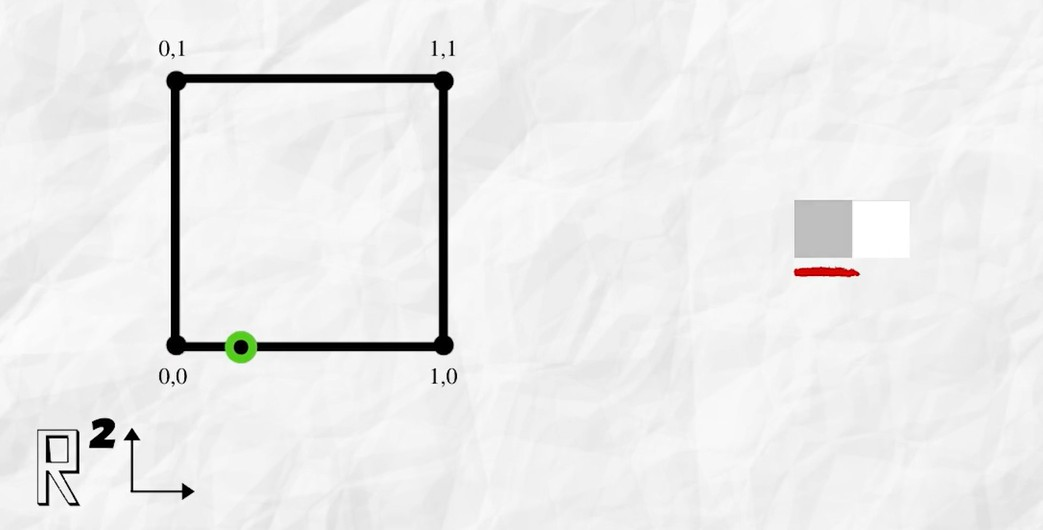
\includegraphics[width=0.45\linewidth,keepaspectratio]{gdl17}
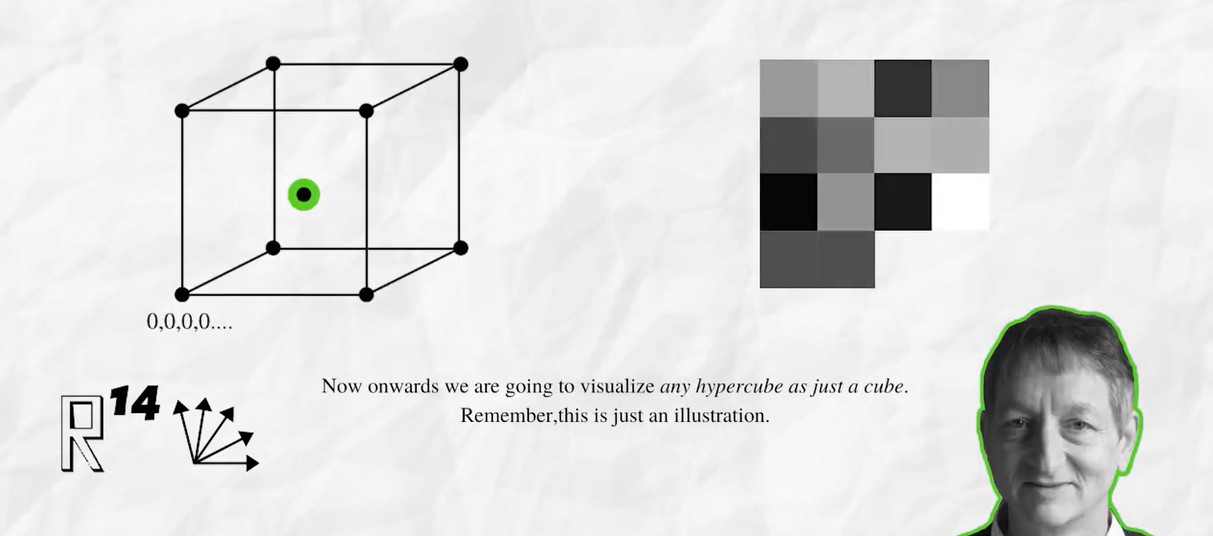
\includegraphics[width=0.45\linewidth,keepaspectratio]{gdl18}

{\tiny (Ref: My Understanding of the Manifold Hypothesis - Kartik Chincholikar)}	

\end{center}

\end{frame}

%%%%%%%%%%%%%%%%%%%%%%%%%%%%%%%%%%%%%%%%%%%%%%%%%%%%%%%%%%%
\begin{frame}[fragile]\frametitle{Images as Points in a Hypercube}
    \begin{itemize}
        \item A grayscale image = point in a high-dimensional space.
        \item 256×256 images, each pixel is a dimension.
        \item All images are just rare points in this vast space.
        \item Random points mostly lead to noise, not meaningful images.
		\item So, only some points in this high dimensional (hyper) space are valid images.
    \end{itemize}
	
\begin{center}
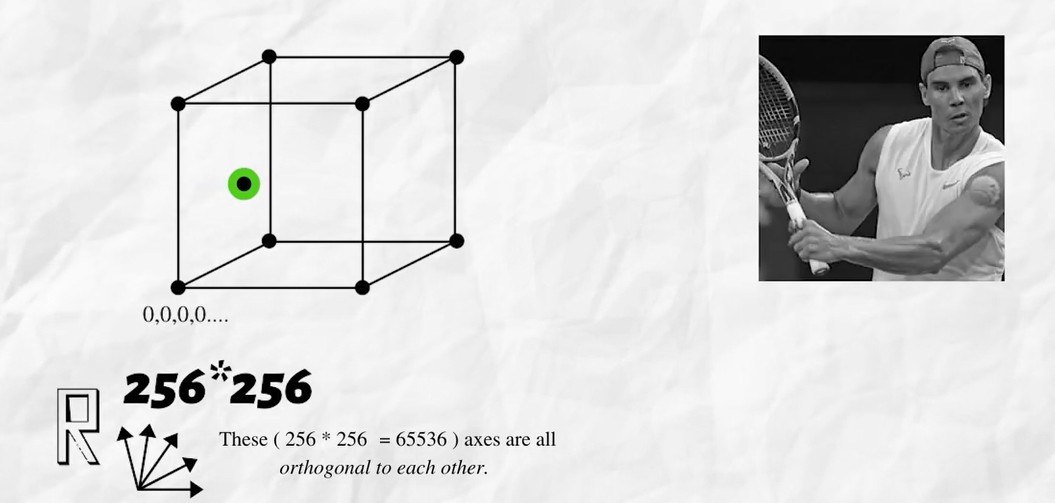
\includegraphics[width=0.5\linewidth,keepaspectratio]{gdl19}

{\tiny (Ref: My Understanding of the Manifold Hypothesis - Kartik Chincholikar)}	

\end{center}	
\end{frame}

%%%%%%%%%%%%%%%%%%%%%%%%%%%%%%%%%%%%%%%%%%%%%%%%%%%%%%%%%%%
\begin{frame}[fragile]\frametitle{Transition Between Images}
    \begin{itemize}
        \item Linear interpolation between points (images) is often not smooth. That gives wierd images.
        \item Intermediate points may not resemble real faces.
        \item Smooth transitions exist along special curved paths, where all are valid images.
        \item These paths lie on the image manifold. E.g. path between morphing from smiling face  to a non-smiling face. Intermediate points are also valid faces.
    \end{itemize}
	
\begin{center}
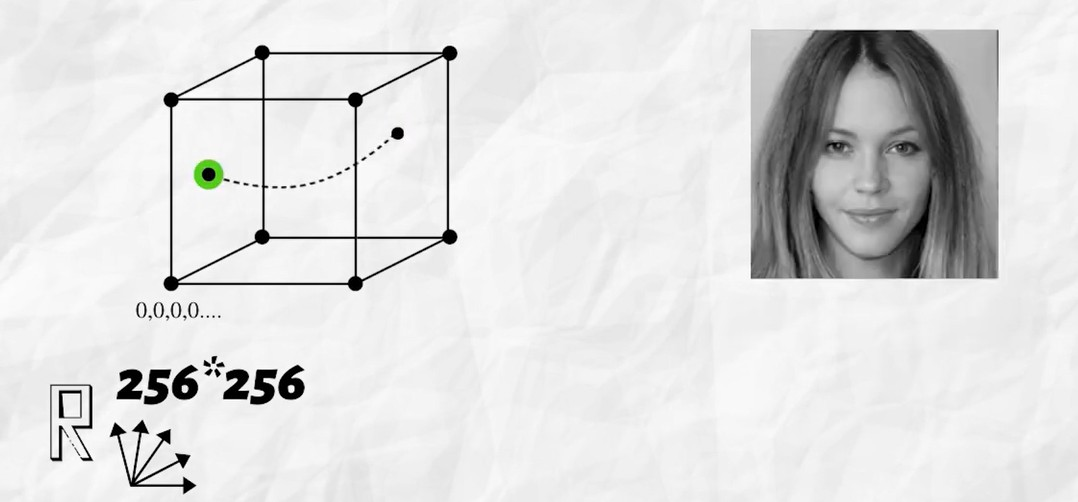
\includegraphics[width=0.5\linewidth,keepaspectratio]{gdl20}

{\tiny (Ref: My Understanding of the Manifold Hypothesis - Kartik Chincholikar)}	

\end{center}	


\end{frame}

%%%%%%%%%%%%%%%%%%%%%%%%%%%%%%%%%%%%%%%%%%%%%%%%%%%%%%%%%%%
\begin{frame}[fragile]\frametitle{Understanding the Face Manifold}
    \begin{itemize}
        \item Each realistic face image lies on or near a manifold.
        \item Moving on the manifold changes expressions smoothly.
        \item Moving off the manifold leads to unrealistic images.
        \item Faces = low-dimensional structure in high-dimensional space, aka Parametric Space that's one dimensional manifold versus 2 dimensional Model or Image space.
    \end{itemize}
	
\begin{center}
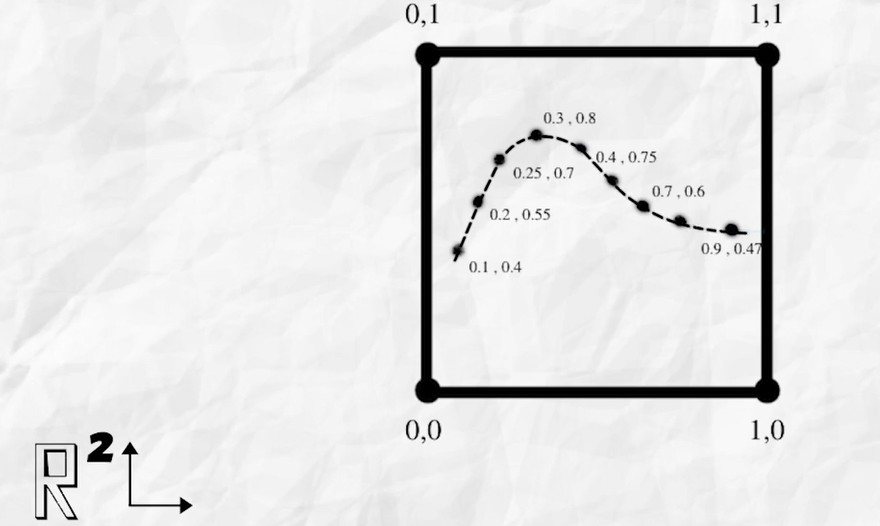
\includegraphics[width=0.5\linewidth,keepaspectratio]{gdl21}

{\tiny (Ref: My Understanding of the Manifold Hypothesis - Kartik Chincholikar)}	

\end{center}		
\end{frame}

%%%%%%%%%%%%%%%%%%%%%%%%%%%%%%%%%%%%%%%%%%%%%%%%%%%%%%%%%%%
\begin{frame}[fragile]\frametitle{Manifolds in Ambient Space}
    \begin{itemize}
        \item Data may lie on a 1D manifold in a 2D space. Underlying geometry.
        \item Example: points following a curved line.
        \item Manifolds are homeomorphic to lower-dimensional Euclidean space.
        \item Local coordinates suffice for representation. Rest of the data is all noise.
    \end{itemize}
	
\begin{center}
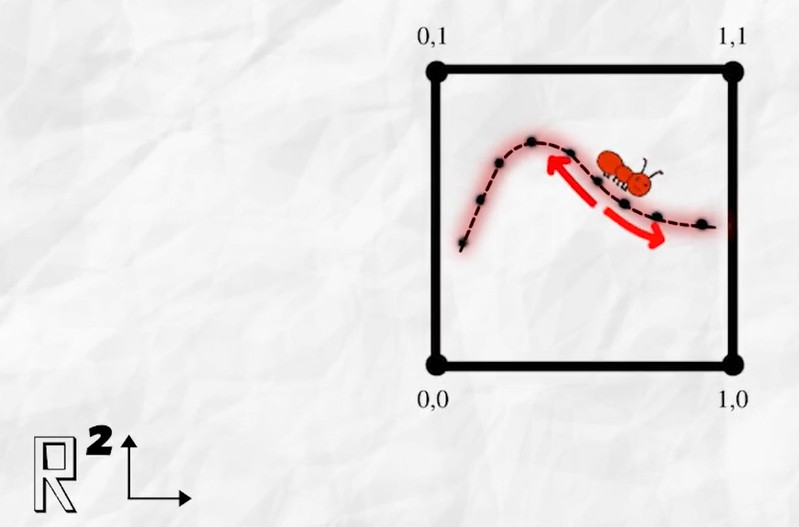
\includegraphics[width=0.5\linewidth,keepaspectratio]{gdl22}

{\tiny (Ref: My Understanding of the Manifold Hypothesis - Kartik Chincholikar)}	

\end{center}
\end{frame}

%%%%%%%%%%%%%%%%%%%%%%%%%%%%%%%%%%%%%%%%%%%%%%%%%%%%%%%%%%%
\begin{frame}[fragile]\frametitle{Degrees of Freedom and Natural Data}
    \begin{itemize}
        \item Real-world data has constraints: limited degrees of freedom.
        \item Example: height vs. weight correlation in humans.
        \item Physical laws restrict images: no cubic planets or levitating people.
        \item Natural images cluster on specific manifolds.
    \end{itemize}
	
\begin{center}
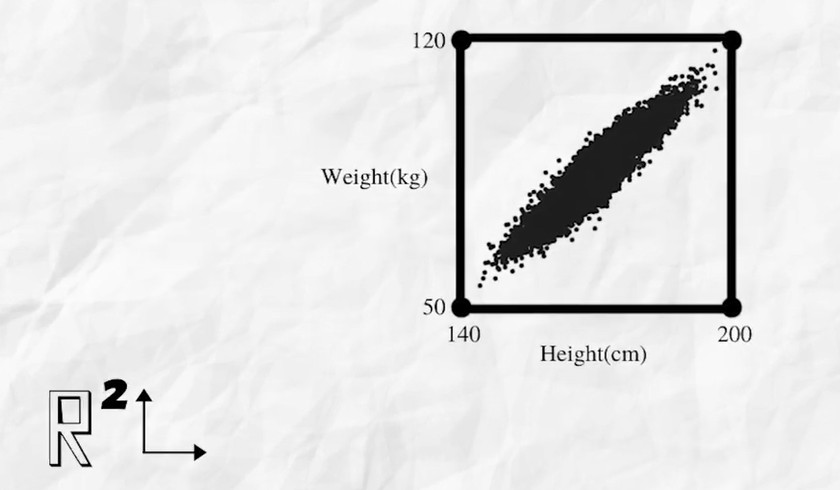
\includegraphics[width=0.5\linewidth,keepaspectratio]{gdl23}

{\tiny (Ref: My Understanding of the Manifold Hypothesis - Kartik Chincholikar)}	

\end{center}	
\end{frame}

%%%%%%%%%%%%%%%%%%%%%%%%%%%%%%%%%%%%%%%%%%%%%%%%%%%%%%%%%%%
\begin{frame}[fragile]\frametitle{Exploring Manifolds Visually}
    \begin{itemize}
        \item Moving on a manifold preserves realistic image features.
        \item Deviating from the manifold introduces noise or anomalies.
        \item Clock images example: midpoints on/off manifold differ significantly.
        \item On-manifold interpolation leads to plausible results.
    \end{itemize}
	
\begin{center}
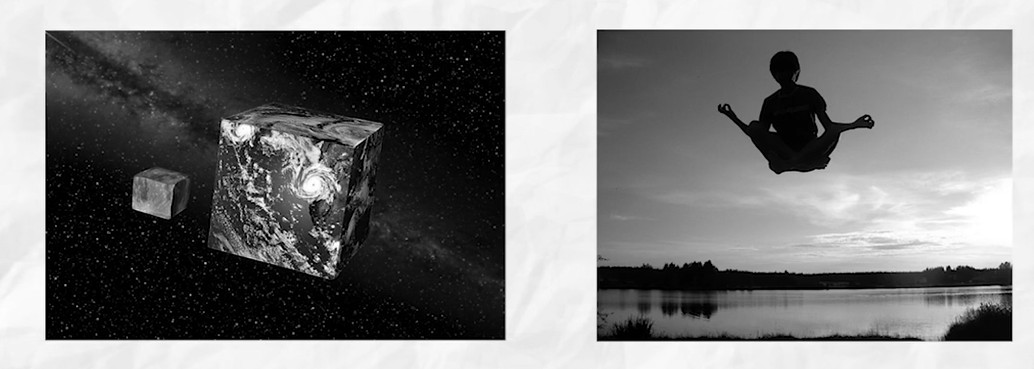
\includegraphics[width=0.7\linewidth,keepaspectratio]{gdl24}

{\tiny (Ref: My Understanding of the Manifold Hypothesis - Kartik Chincholikar)}	

\end{center}		
\end{frame}

%%%%%%%%%%%%%%%%%%%%%%%%%%%%%%%%%%%%%%%%%%%%%%%%%%%%%%%%%%%
\begin{frame}[fragile]\frametitle{Learning the Manifold}
    \begin{itemize}
        \item ML models aim to approximate data manifolds.
        \item VAEs and GANs learn mappings from latent to pixel space.
        \item Latent space is low-dimensional, manifold is high-dimensional.
        \item Models learn this mapping via optimization, not manual rules.
    \end{itemize}
	
\begin{center}
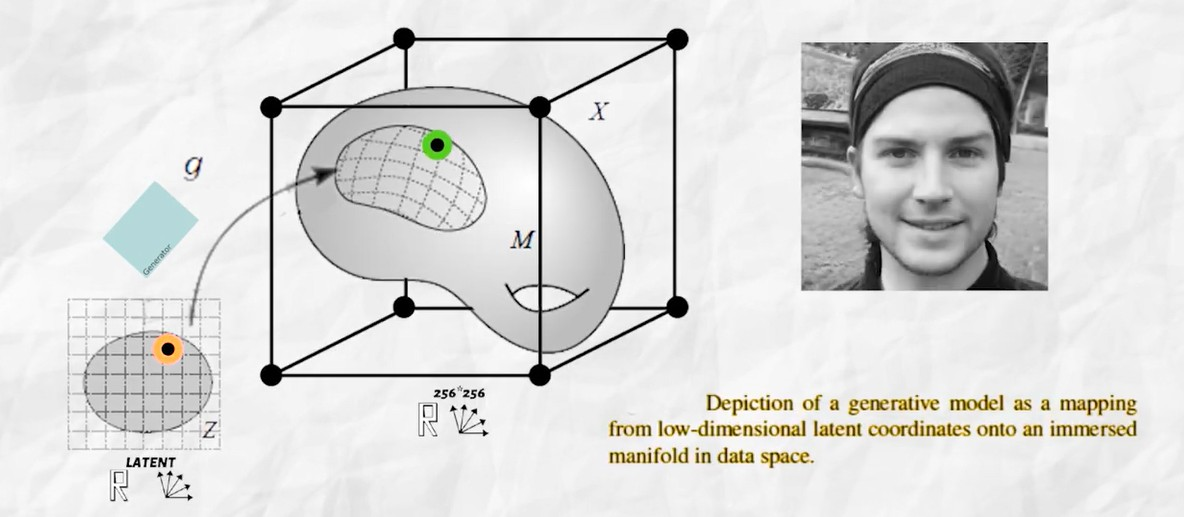
\includegraphics[width=0.5\linewidth,keepaspectratio]{gdl25}

{\tiny (Ref: My Understanding of the Manifold Hypothesis - Kartik Chincholikar)}	

\end{center}	
\end{frame}

%%%%%%%%%%%%%%%%%%%%%%%%%%%%%%%%%%%%%%%%%%%%%%%%%%%%%%%%%%%
\begin{frame}[fragile]\frametitle{Control and Future Directions}
    \begin{itemize}
        \item Better control of latent features is an active research area.
        \item Goal: steer generation with interpretable latent directions.
        \item Understanding manifolds improves generative model performance.
    \end{itemize}
\end{frame}

%%%%%%%%%%%%%%%%%%%%%%%%%%%%%%%%%%%%%%%%%%%%%%%%%%%%%%%%%%%%%%%%%%%%%%%%%%%%%%%%%%
\begin{frame}[fragile]\frametitle{}
\begin{center}
{\Large Manifold vs Graph}
\end{center}
\end{frame}

%%%%%%%%%%%%%%%%%%%%%%%%%%%%%%%%%%%%%%%%%%%%%%%%%%%%%%%%%%%
\begin{frame}[fragile]\frametitle{Manifolds vs. Graphs: Basic Idea}
    \begin{itemize}
        \item Manifolds are continuous spaces that locally resemble Euclidean space.
        \item Graphs are discrete structures made of nodes and edges.
        \item Manifolds generalize smooth surfaces and curves.
        \item Graphs represent relationships or connections in data.
    \end{itemize}
\end{frame}

%%%%%%%%%%%%%%%%%%%%%%%%%%%%%%%%%%%%%%%%%%%%%%%%%%%%%%%%%%%
\begin{frame}[fragile]\frametitle{What is a Manifold?}
    \begin{itemize}
        \item A manifold locally looks like \(\mathbb{R}^n\), the Euclidean space.
        \item Every small neighborhood on the manifold is flat.
        \item Tangent space and curvature can be defined on smooth manifolds.
        \item Common in geometry, physics, and ML.
    \end{itemize}
\end{frame}

%%%%%%%%%%%%%%%%%%%%%%%%%%%%%%%%%%%%%%%%%%%%%%%%%%%%%%%%%%%
\begin{frame}[fragile]\frametitle{Examples of Manifolds}
    \begin{itemize}
        \item A sphere is a 2D manifold—locally flat, globally curved.
        \item A torus (donut surface) is also a 2D manifold.
        \item Any surface where local patches resemble \(\mathbb{R}^2\).
    \end{itemize}
\end{frame}

%%%%%%%%%%%%%%%%%%%%%%%%%%%%%%%%%%%%%%%%%%%%%%%%%%%%%%%%%%%
\begin{frame}[fragile]\frametitle{What is a Graph?}
    \begin{itemize}
        \item Graphs consist of vertices (nodes) and edges (links).
        \item No notion of continuity or smoothness.
        \item Structure depends on how nodes are connected.
        \item Used to represent social networks, maps, trees, etc.
    \end{itemize}
\end{frame}

%%%%%%%%%%%%%%%%%%%%%%%%%%%%%%%%%%%%%%%%%%%%%%%%%%%%%%%%%%%
\begin{frame}[fragile]\frametitle{Examples of Graphs}
    \begin{itemize}
        \item Social network: users are nodes, friendships are edges.
        \item Road maps: cities as nodes, roads as edges.
        \item Family trees: people as nodes, lineage as edges.
    \end{itemize}
\end{frame}

%%%%%%%%%%%%%%%%%%%%%%%%%%%%%%%%%%%%%%%%%%%%%%%%%%%%%%%%%%%
\begin{frame}[fragile]\frametitle{Key Differences}
    \begin{itemize}
        \item Manifolds are continuous; graphs are discrete.
        \item Manifolds often support calculus; graphs don't.
        \item Manifolds have local Euclidean charts; graphs have neighborhoods.
        \item Different math tools: topology vs. graph theory.
    \end{itemize}
\end{frame}

%%%%%%%%%%%%%%%%%%%%%%%%%%%%%%%%%%%%%%%%%%%%%%%%%%%%%%%%%%%
\begin{frame}[fragile]\frametitle{Connecting Manifolds and Graphs}
    \begin{itemize}
        \item Graphs can approximate manifolds in data analysis.
        \item Manifolds can be seen as continuous analogs of graphs.
        \item Concepts can sometimes translate between the two.
    \end{itemize}
\end{frame}

%%%%%%%%%%%%%%%%%%%%%%%%%%%%%%%%%%%%%%%%%%%%%%%%%%%%%%%%%%%
\begin{frame}[fragile]\frametitle{Applications of Manifolds}
    \begin{itemize}
        \item Used in differential geometry and general relativity.
        \item Describe smooth, high-dimensional data in ML.
        \item Essential in algorithms like PCA, LLE, and t-SNE.
    \end{itemize}
\end{frame}

%%%%%%%%%%%%%%%%%%%%%%%%%%%%%%%%%%%%%%%%%%%%%%%%%%%%%%%%%%%
\begin{frame}[fragile]\frametitle{Applications of Graphs}
    \begin{itemize}
        \item Data structures in computer science and AI.
        \item Modeling networks: internet, traffic, biology.
        \item Powering algorithms like PageRank, graph neural networks.
    \end{itemize}
\end{frame}


%%%%%%%%%%%%%%%%%%%%%%%%%%%%%%%%%%%%%%%%%%%%%%%%%%%%%%%%%%%%%%%%%%%%%%%%%%%%%%%%%%
\begin{frame}[fragile]\frametitle{}
\begin{center}
{\Large Geometric Deep Learning: From Grids to Gauges}
\vspace{0.5cm}

{\em Unifying Neural Architectures Through Geometric Principles}
\end{center}
\end{frame}

%%%%%%%%%%%%%%%%%%%%%%%%%%%%%%%%%%%%%%%%%%%%%%%%%%%%%%%%%%%%%%%%%%%%%%%%%%%%%%%%%%
\begin{frame}[fragile]\frametitle{The Fundamental Challenge}

\begin{center}
\textbf{Why do we need so many different neural network architectures?}
\end{center}

\begin{columns}
\begin{column}{0.5\textwidth}
\begin{itemize}
\item MLPs: Tabular data
\item CNNs: Images 
\item RNNs: Sequences
\item Transformers: Sets with attention
\item GNNs: Graphs
\end{itemize}
\end{column}
\begin{column}{0.5\textwidth}
\begin{center}
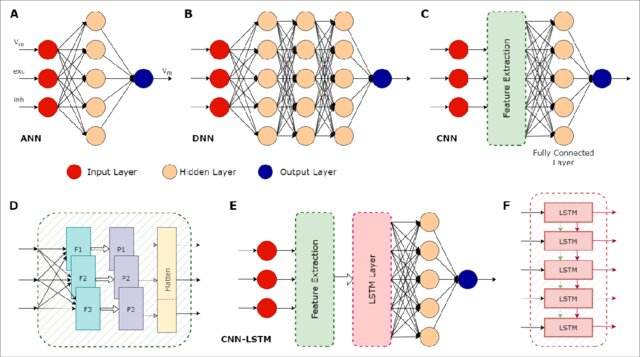
\includegraphics[width=\linewidth]{architectures_evolution}
\end{center}
\end{column}
\end{columns}

\vspace{0.5cm}
\begin{alertblock}{Key Insight}
Each architecture encodes specific \textbf{geometric assumptions} about the data structure!
\end{alertblock}

\end{frame}

%%%%%%%%%%%%%%%%%%%%%%%%%%%%%%%%%%%%%%%%%%%%%%%%%%%%%%%%%%%%%%%%%%%%%%%%%%%%%%%%%%
\begin{frame}[fragile]\frametitle{Data Has Shape, Shape Has Meaning}

\begin{center}
\begin{tabular}{|c|c|c|c|}
\hline
\textbf{Data Type} & \textbf{Structure} & \textbf{Key Property} & \textbf{Architecture} \\
\hline
Tabular & Fixed vectors & Independence & MLP \\
Images & Regular grid & Translation & CNN \\
Sequences & 1D chain & Order & RNN \\
Sets & Unordered & Permutation & Attention \\
Graphs & Irregular & Connectivity & GNN \\
\hline
\end{tabular}
\end{center}

\vspace{0.5cm}

\begin{block}{The Geometric Deep Learning Hypothesis}
\begin{center}
\textbf{The success of a neural architecture is determined by how well its geometric biases match the geometric structure of the data.}
\end{center}
\end{block}

\end{frame}

%%%%%%%%%%%%%%%%%%%%%%%%%%%%%%%%%%%%%%%%%%%%%%%%%%%%%%%%%%%%%%%%%%%%%%%%%%%%%%%%%%
\begin{frame}[fragile]\frametitle{Felix Klein's Vision: The Erlangen Program (1872)}

\begin{columns}
\begin{column}{0.6\textwidth}
\textbf{Klein's Revolutionary Idea:}
\begin{itemize}
\item Classify geometries by their \textbf{symmetry groups}
\item A geometry = invariant properties under transformations
\item Unified framework for all geometric spaces
\end{itemize}

\vspace{0.5cm}
\textbf{Modern Translation:}
\begin{itemize}
\item Classify neural networks by their \textbf{equivariances}
\item An architecture = invariant computations under transformations  
\item Unified framework for all data domains
\end{itemize}
\end{column}
\begin{column}{0.4\textwidth}
\begin{center}
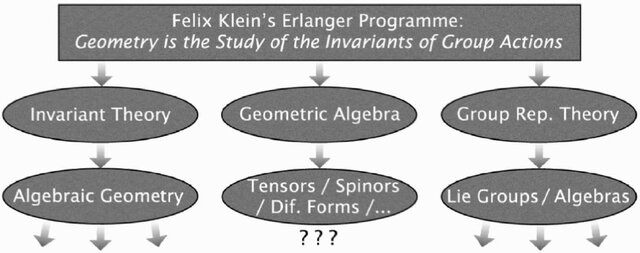
\includegraphics[width=\linewidth]{klein_program}

\vspace{0.5cm}
{\small "Geometry is the study of invariant properties under group actions"}
\end{center}
\end{column}
\end{columns}

\end{frame}

%%%%%%%%%%%%%%%%%%%%%%%%%%%%%%%%%%%%%%%%%%%%%%%%%%%%%%%%%%%%%%%%%%%%%%%%%%%%%%%%%%
\begin{frame}[fragile]\frametitle{The 5G Framework: Grids, Groups, Graphs, Geodesics, Gauges}

\begin{center}
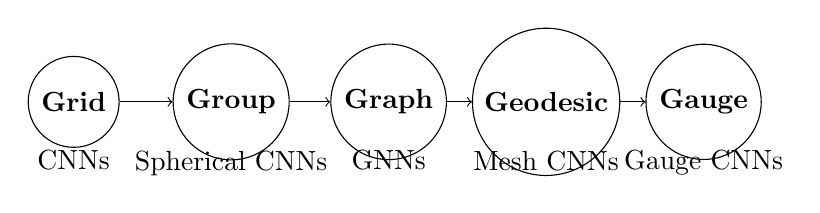
\begin{tikzpicture}
\node[draw,circle,minimum size=1cm] (grid) at (0,0) {\textbf{Grid}};
\node[draw,circle,minimum size=1cm] (group) at (2,0) {\textbf{Group}};
\node[draw,circle,minimum size=1cm] (graph) at (4,0) {\textbf{Graph}};
\node[draw,circle,minimum size=1cm] (geodesic) at (6,0) {\textbf{Geodesic}};
\node[draw,circle,minimum size=1cm] (gauge) at (8,0) {\textbf{Gauge}};

\draw[->] (grid) -- (group);
\draw[->] (group) -- (graph);
\draw[->] (graph) -- (geodesic);
\draw[->] (geodesic) -- (gauge);

\node[below=0.5cm] at (0,0) {CNNs};
\node[below=0.5cm] at (2,0) {Spherical CNNs};
\node[below=0.5cm] at (4,0) {GNNs};
\node[below=0.5cm] at (6,0) {Mesh CNNs};
\node[below=0.5cm] at (8,0) {Gauge CNNs};
\end{tikzpicture}
\end{center}

\vspace{0.5cm}

\begin{block}{Progression of Geometric Complexity}
\begin{itemize}
\item \textbf{Grid}: Regular lattices (images) → Translation equivariance
\item \textbf{Group}: Homogeneous spaces (sphere) → Group equivariance  
\item \textbf{Graph}: Discrete structures → Permutation invariance
\item \textbf{Geodesic}: Continuous manifolds → Diffeomorphism invariance
\item \textbf{Gauge}: Vector bundles → Gauge equivariance
\end{itemize}
\end{block}

\end{frame}

%%%%%%%%%%%%%%%%%%%%%%%%%%%%%%%%%%%%%%%%%%%%%%%%%%%%%%%%%%%%%%%%%%%%%%%%%%%%%%%%%%
\begin{frame}[fragile]\frametitle{From Invariance to Equivariance}

\begin{columns}
\begin{column}{0.5\textwidth}
\textbf{Invariance:} Output unchanged
$$f(g \cdot x) = f(x)$$

\textbf{Equivariance:} Output transforms predictably  
$$f(g \cdot x) = \rho(g) \cdot f(x)$$

where $g \in G$ (group), $\rho$ is representation
\end{column}
\begin{column}{0.5\textwidth}
% \begin{center}
% \includegraphics[width=\linewidth]{invariance_equivariance}
% \end{center}
\end{column}
\end{columns}

\vspace{0.5cm}

\begin{exampleblock}{CNN Translation Equivariance}
If we translate input image → CNN features translate by same amount

\texttt{conv(translate(image)) = translate(conv(image))}
\end{exampleblock}

\begin{alertblock}{Why Equivariance > Invariance?}
Equivariance preserves spatial relationships, enabling hierarchical processing
\end{alertblock}

\end{frame}

%%%%%%%%%%%%%%%%%%%%%%%%%%%%%%%%%%%%%%%%%%%%%%%%%%%%%%%%%%%%%%%%%%%%%%%%%%%%%%%%%%
\begin{frame}[fragile]\frametitle{The Permutation Challenge}

\begin{center}
\textbf{Consider a set $\{A, B, C\}$ - How many ways to order it?}
\end{center}

\begin{columns}
\begin{column}{0.35\textwidth}
\textbf{All permutations:}
\begin{itemize}
\item $\{A, B, C\}$
\item $\{A, C, B\}$  
\item $\{B, A, C\}$
\item $\{B, C, A\}$
\item $\{C, A, B\}$
\item $\{C, B, A\}$
\end{itemize}

\textbf{Total: $3! = 6$ orderings}
\end{column}
\begin{column}{0.65\textwidth}
\textbf{Traditional ML approach:}
\begin{itemize}
\item Learn function for each ordering
\item Requires 6× more data
\item No generalization across orderings
\end{itemize}

\vspace{0.2cm}
\textbf{Geometric ML approach:}
\begin{itemize}
\item Learn \textbf{permutation invariant} function
\item Same function works for all orderings
\item Dramatic sample efficiency gain
\end{itemize}
\end{column}
\end{columns}

\begin{block}{Mathematical Formulation}
$$f(\pi \cdot X) = f(X) \quad \forall \pi \in S_n$$
where $\pi$ is any permutation, $S_n$ is symmetric group
\end{block}

\end{frame}

%%%%%%%%%%%%%%%%%%%%%%%%%%%%%%%%%%%%%%%%%%%%%%%%%%%%%%%%%%%%%%%%%%%%%%%%%%%%%%%%%%
\begin{frame}[fragile]\frametitle{Grid Domain: CNNs and Translation Equivariance}

\begin{center}
\textbf{Regular Grid Structure}
\end{center}

\begin{columns}
\begin{column}{0.6\textwidth}
\textbf{Key Properties:}
\begin{itemize}
\item Fixed neighborhood structure
\item Translation symmetry
\item Local connectivity
\item Regular sampling
\end{itemize}

% \vspace{0.5cm}
\textbf{CNN Operation:}
$$(\mathbf{f} * \mathbf{g})[i,j] = \sum_{m,n} \mathbf{f}[m,n] \cdot \mathbf{g}[i-m, j-n]$$

\textbf{Equivariance Property:}
$$\text{Conv}(T_v(\mathbf{x})) = T_v(\text{Conv}(\mathbf{x}))$$
\end{column}
\begin{column}{0.4\textwidth}
\begin{center}
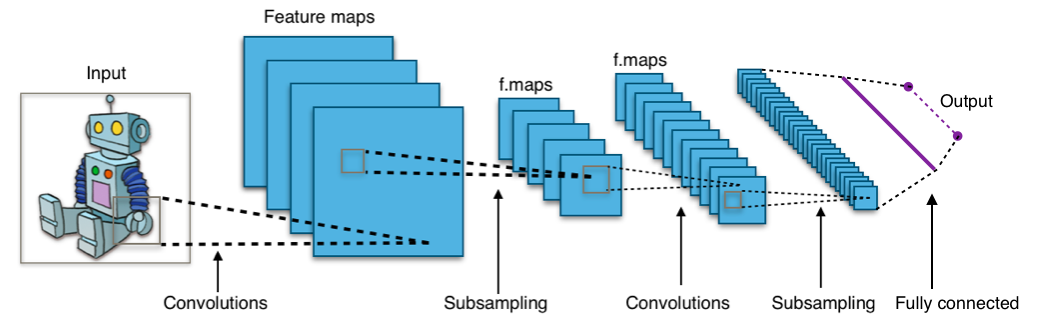
\includegraphics[width=\linewidth]{cnn_grid}

\vspace{0.5cm}
{\small Convolution preserves spatial relationships}
\end{center}
\end{column}
\end{columns}

\begin{alertblock}{Limitation}
CNNs fail on irregular, non-grid data (graphs, point clouds, meshes)
\end{alertblock}

\end{frame}

%%%%%%%%%%%%%%%%%%%%%%%%%%%%%%%%%%%%%%%%%%%%%%%%%%%%%%%%%%%%%%%%%%%%%%%%%%%%%%%%%%
\begin{frame}[fragile]\frametitle{Group Domain: Beyond Translation}

\begin{center}
\textbf{Homogeneous Spaces with Global Symmetries}
\end{center}

\begin{columns}
\begin{column}{0.5\textwidth}
\textbf{Examples:}
\begin{itemize}
\item \textbf{Sphere}: $SO(3)$ rotations
\item \textbf{Scale space}: Scaling transformations  
\item \textbf{Roto-translation}: $SE(2)$ group
\end{itemize}

% \vspace{0.5cm}
\textbf{Group Convolution:}
$$[f *_G \psi](g) = \int_G f(h) \psi(g^{-1}h) dh$$

\textbf{Applications:}
\begin{itemize}
\item Spherical CNNs for 360° images
\item Scale-equivariant networks
\item Rotation-invariant vision
\end{itemize}
\end{column}
\begin{column}{0.5\textwidth}
\begin{center}
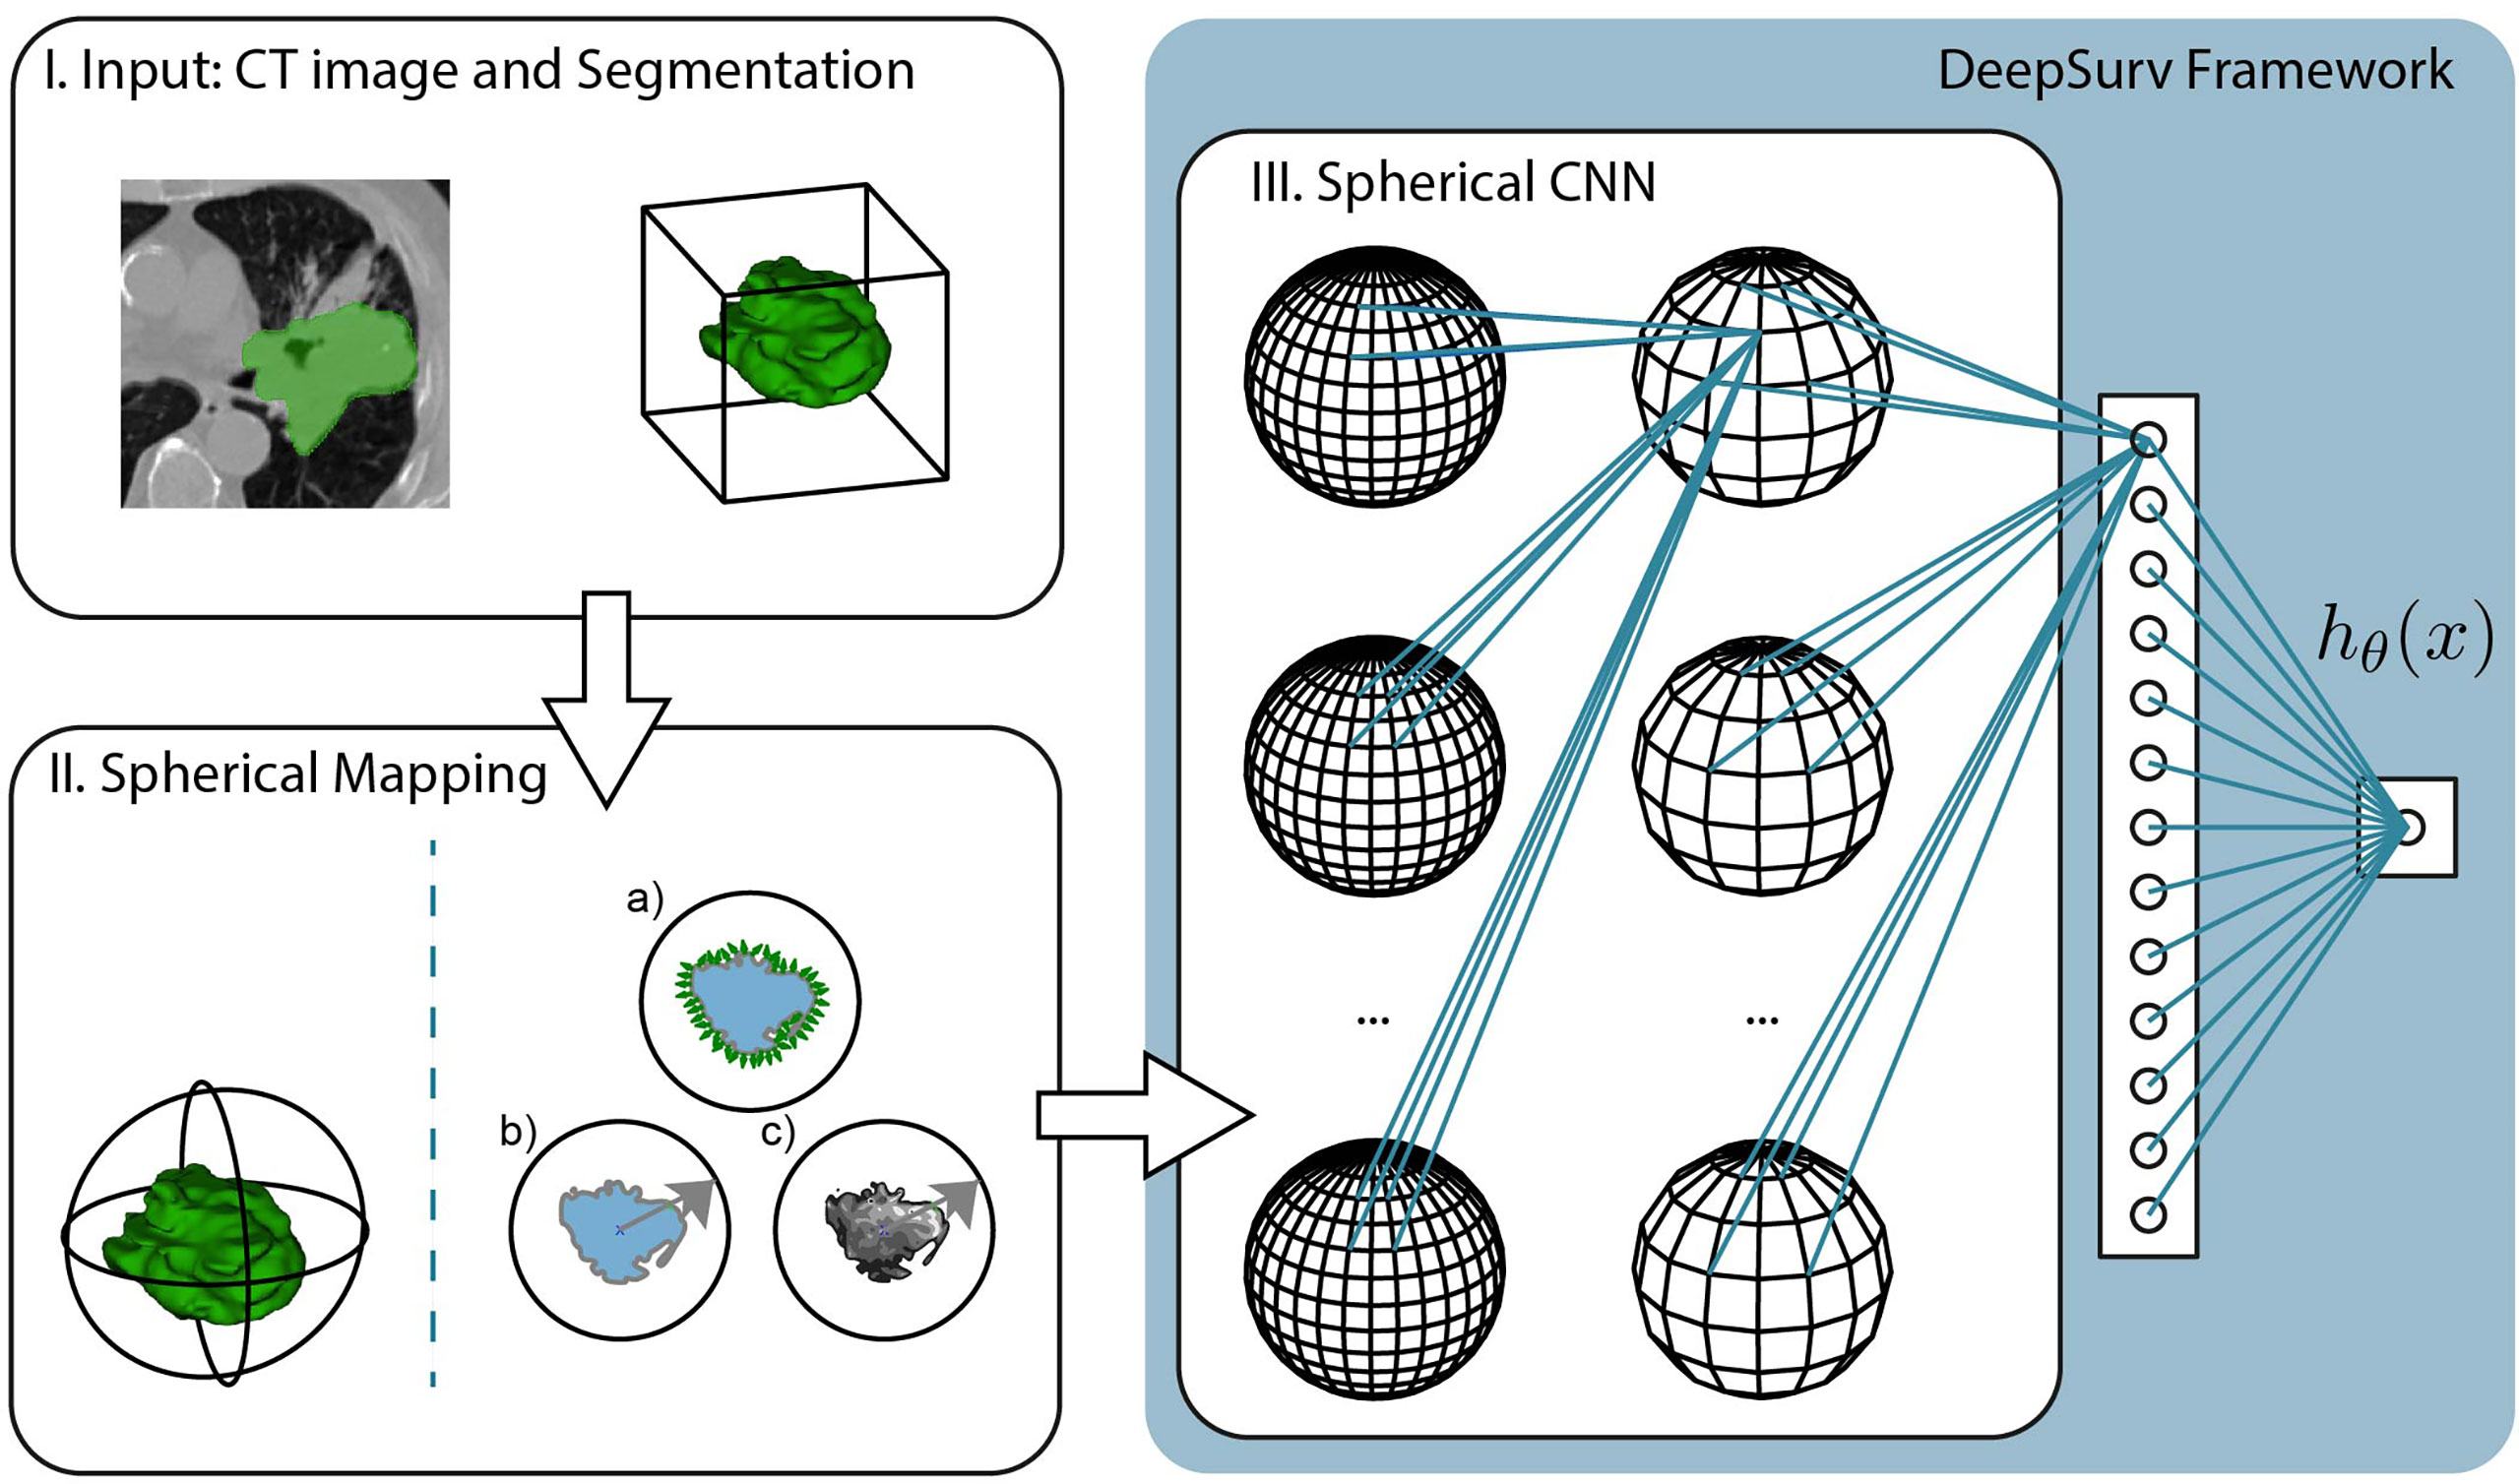
\includegraphics[width=\linewidth]{spherical_cnn}

\vspace{0.5cm}
{\small Spherical convolution on global data}
\end{center}
\end{column}
\end{columns}

\begin{block}{Key Insight}
Group equivariance generalizes translation equivariance to richer symmetries
\end{block}

\end{frame}

%%%%%%%%%%%%%%%%%%%%%%%%%%%%%%%%%%%%%%%%%%%%%%%%%%%%%%%%%%%%%%%%%%%%%%%%%%%%%%%%%%
\begin{frame}[fragile]\frametitle{Graph Domain: Permutation Invariance}

\begin{center}
\textbf{Irregular Connectivity Structures}
\end{center}

\begin{columns}
\begin{column}{0.6\textwidth}
\textbf{Key Challenges:}
\begin{itemize}
\item Variable node degrees
\item No canonical ordering
\item Irregular neighborhoods
\item Arbitrary connectivity patterns
\end{itemize}

% \vspace{0.5cm}
\textbf{Graph Convolution:}
$$\mathbf{H}^{(l+1)} = \sigma\left(\mathbf{D}^{-\frac{1}{2}}\mathbf{A}\mathbf{D}^{-\frac{1}{2}}\mathbf{H}^{(l)}\mathbf{W}^{(l)}\right)$$


\end{column}
\begin{column}{0.4\textwidth}
{\small Graph with irregular connectivity}

\begin{center}
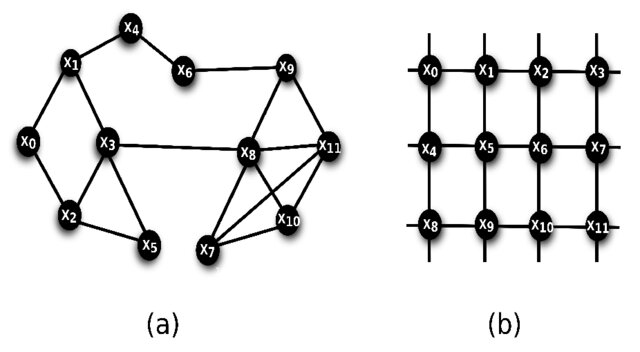
\includegraphics[width=\linewidth]{graph_structure}
\end{center}

\textbf{Permutation Invariance:}
$$f(\mathbf{P}\mathbf{X}, \mathbf{P}\mathbf{A}\mathbf{P}^T) = f(\mathbf{X}, \mathbf{A})$$
\end{column}
\end{columns}

\begin{exampleblock}{Message Passing Framework}
$$\mathbf{m}_{ij}^{(l)} = M^{(l)}(\mathbf{h}_i^{(l)}, \mathbf{h}_j^{(l)}, \mathbf{e}_{ij})$$
$$\mathbf{h}_i^{(l+1)} = U^{(l)}\left(\mathbf{h}_i^{(l)}, \text{AGG}\left(\{\mathbf{m}_{ij}^{(l)} : j \in \mathcal{N}(i)\}\right)\right)$$
\end{exampleblock}

\end{frame}

%%%%%%%%%%%%%%%%%%%%%%%%%%%%%%%%%%%%%%%%%%%%%%%%%%%%%%%%%%%%%%%%%%%%%%%%%%%%%%%%%%
\begin{frame}[fragile]\frametitle{Geodesic Domain: Manifold Learning}

\begin{center}
\textbf{Continuous Curved Spaces}
\end{center}

\begin{columns}
\begin{column}{0.4\textwidth}
\textbf{Key Concepts:}
\begin{itemize}
\item Riemannian manifolds
\item Geodesic distances
\item Intrinsic geometry
\item Curvature effects
\end{itemize}

% \vspace{0.5cm}

\textbf{Applications:}
\begin{itemize}
\item 3D shape analysis
\item Molecular surfaces
\item Brain cortex modeling
\end{itemize}
\end{column}
\begin{column}{0.6\textwidth}
{\small 3D mesh with geodesic paths}

\begin{center}
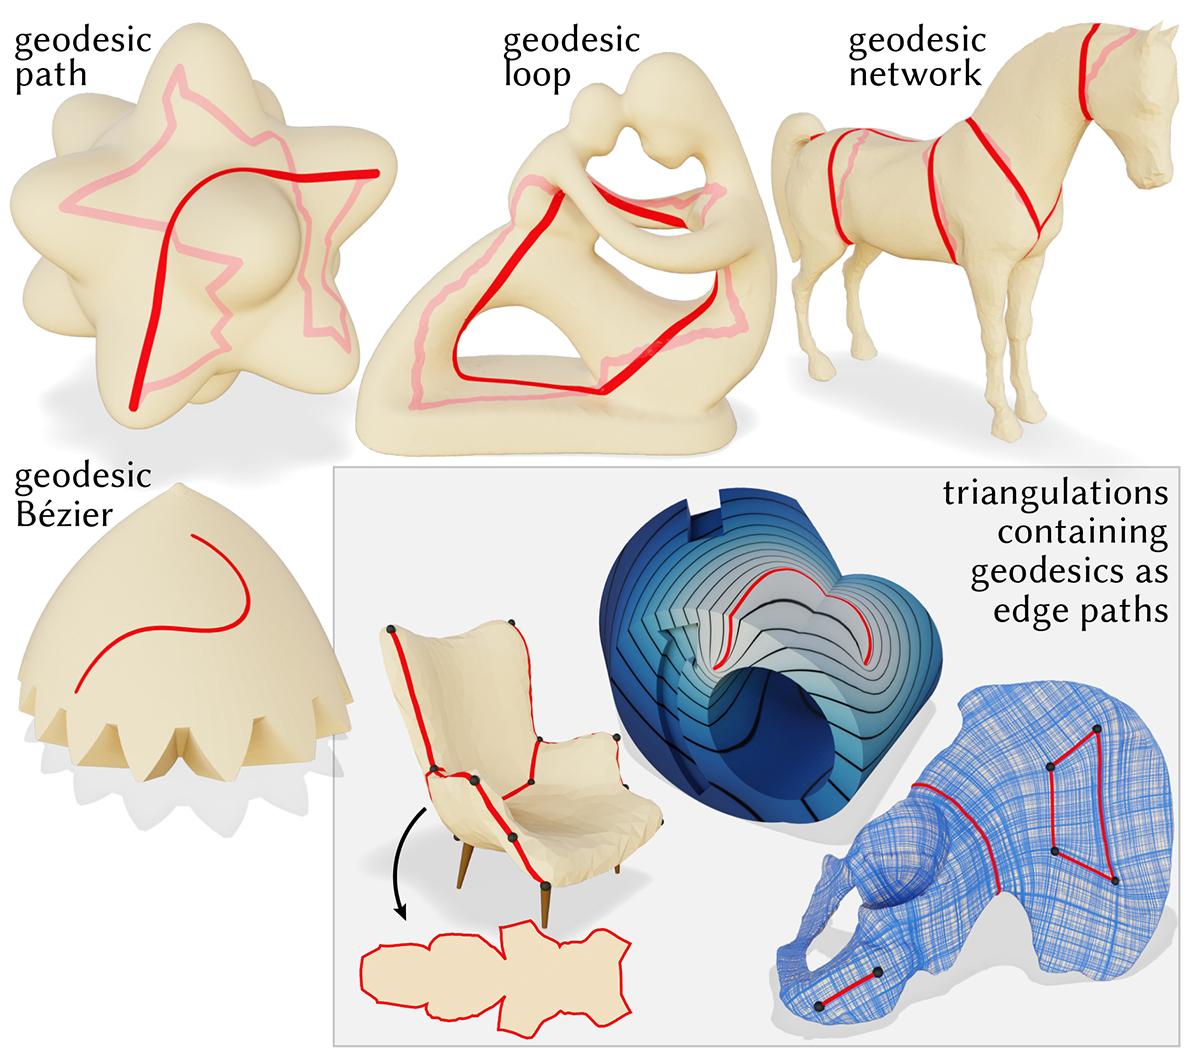
\includegraphics[width=0.5\linewidth]{manifold_mesh}
\end{center}

\textbf{Geodesic Convolution:}
$$[f * \psi]_{\mathcal{M}}(x) = \int_{\mathcal{M}} f(y) \psi(d_{\mathcal{M}}(x,y)) d\mu(y)$$

\end{column}
\end{columns}

\begin{block}{Diffeomorphism Invariance}
Functions invariant to smooth, invertible deformations of the manifold
\end{block}

\end{frame}

%%%%%%%%%%%%%%%%%%%%%%%%%%%%%%%%%%%%%%%%%%%%%%%%%%%%%%%%%%%%%%%%%%%%%%%%%%%%%%%%%%
\begin{frame}[fragile]\frametitle{Gauge Domain: Vector Bundles}

\begin{center}
\textbf{Most General Geometric Structure}
\end{center}


\textbf{Key Concepts:}
\begin{itemize}
\item Vector bundles over manifolds
\item Gauge transformations
\item Connection and curvature
\item Parallel transport
\end{itemize}

% \vspace{0.5cm}
\textbf{Gauge Equivariant Convolution:}
$$[f *_{\text{gauge}} \psi](x) = \int_{\mathcal{M}} \Phi(x,y) f(y) \psi(x,y) d\mu(y)$$

where $\Phi(x,y)$ is parallel transport operator

\end{frame}


%%%%%%%%%%%%%%%%%%%%%%%%%%%%%%%%%%%%%%%%%%%%%%%%%%%%%%%%%%%%%%%%%%%%%%%%%%%%%%%%%%
\begin{frame}[fragile]\frametitle{Gauge Domain: Vector Bundles}

\begin{columns}
\begin{column}{0.6\textwidth}
\textbf{Applications:}
\begin{itemize}
\item Weather prediction on sphere
\item Fluid dynamics
\item Electromagnetic fields
\end{itemize}
\end{column}
\begin{column}{0.4\textwidth}
\begin{center}
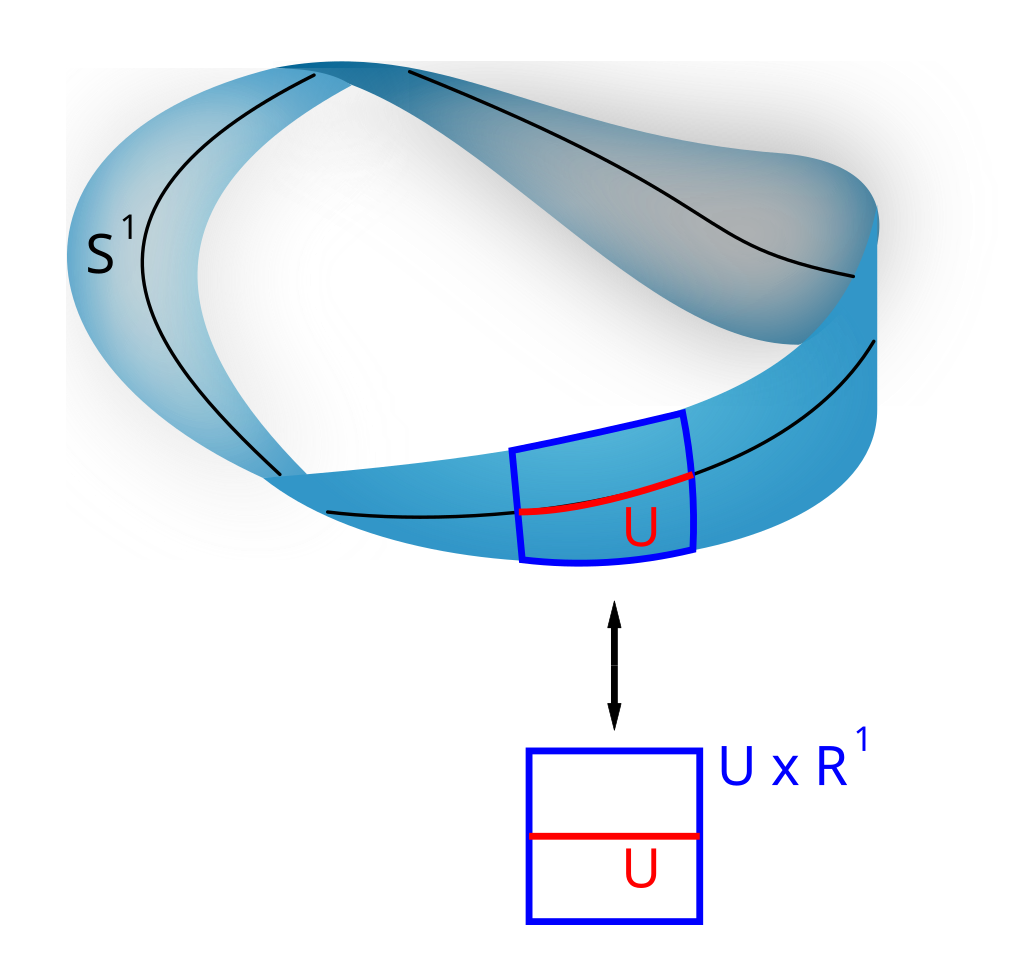
\includegraphics[width=\linewidth]{vector_bundle}

% \vspace{0.5cm}
{\small Vector bundle with gauge connection}
\end{center}
\end{column}
\end{columns}

\begin{alertblock}{Ultimate Generalization}
Gauge networks represent the most general form of geometric deep learning
\end{alertblock}

\end{frame}

%%%%%%%%%%%%%%%%%%%%%%%%%%%%%%%%%%%%%%%%%%%%%%%%%%%%%%%%%%%%%%%%%%%%%%%%%%%%%%%%%%
\begin{frame}[fragile]\frametitle{The Unified Message Passing Framework}

\begin{center}
\textbf{All Geometric Networks Share Common Structure}
\end{center}

\begin{block}{General Message Passing Layer}
\begin{align}
\mathbf{m}_{ij}^{(l)} &= M^{(l)}(\mathbf{h}_i^{(l)}, \mathbf{h}_j^{(l)}, \mathbf{e}_{ij}) \\
\mathbf{h}_i^{(l+1)} &= U^{(l)}\left(\mathbf{h}_i^{(l)}, \text{AGG}\left(\{\mathbf{m}_{ij}^{(l)} : j \in \mathcal{N}(i)\}\right)\right)
\end{align}
\end{block}

\begin{center}
\begin{tabular}{|l|l|l|}
\hline
\textbf{Domain} & \textbf{Neighborhood $\mathcal{N}(i)$} & \textbf{Message Function $M$} \\
\hline
Grid & Fixed spatial neighbors & Convolution kernel \\
Group & Group orbit & Group convolution \\
Graph & Adjacent nodes & Learned function \\
Geodesic & Geodesic neighbors & Distance-based \\
Gauge & Parallel transport & Gauge connection \\
\hline
\end{tabular}
\end{center}

\begin{alertblock}{Universal Framework}
The 5G domains differ only in their definition of neighborhood and message function!
\end{alertblock}

\end{frame}

%%%%%%%%%%%%%%%%%%%%%%%%%%%%%%%%%%%%%%%%%%%%%%%%%%%%%%%%%%%%%%%%%%%%%%%%%%%%%%%%%%
\begin{frame}[fragile]\frametitle{Spectral vs Spatial Graph Convolutions}

\begin{columns}
\begin{column}{0.5\textwidth}
\textbf{Spectral Approach:}
\begin{itemize}
\item Based on graph Fourier transform
\item Uses eigen-decomposition of Laplacian
\item Global receptive field
\item Computationally expensive
\end{itemize}

\textbf{Graph Fourier Transform:}
$\hat{f}(\lambda_i) = \sum_{j=1}^n f(j) u_i(j)$

\textbf{Spectral Convolution:}
$g_\theta * f = U g_\theta(\Lambda) U^T f$
\end{column}
\begin{column}{0.5\textwidth}
\textbf{Spatial Approach:}
\begin{itemize}
\item Direct neighborhood aggregation
\item Local message passing
\item Inductive capability
\item Computationally efficient
\end{itemize}

\textbf{Spatial Convolution:}
$h_i^{(l+1)} = \sigma\left(\sum_{j \in \mathcal{N}(i)} \frac{1}{\sqrt{d_i d_j}} h_j^{(l)} W^{(l)}\right)$
\end{column}
\end{columns}

% \vspace{0.5cm}

\begin{center}
\begin{tabular}{|l|c|c|}
\hline
\textbf{Property} & \textbf{Spectral} & \textbf{Spatial} \\
\hline
Localization & Global & Local \\
Inductive & No & Yes \\
Efficiency & Low & High \\
Interpretability & Mathematical & Intuitive \\
\hline
\end{tabular}
\end{center}

\end{frame}

%%%%%%%%%%%%%%%%%%%%%%%%%%%%%%%%%%%%%%%%%%%%%%%%%%%%%%%%%%%%%%%%%%%%%%%%%%%%%%%%%%
\begin{frame}[fragile]\frametitle{Success Stories Across Domains}

\begin{center}
\textbf{Geometric Deep Learning in Action}
\end{center}

\begin{columns}
\begin{column}{0.5\textwidth}
\textbf{Computer Vision:}
\begin{itemize}
\item Spherical CNNs for 360° video
\item Scale-equivariant detection
\item 3D shape analysis
\end{itemize}

\textbf{Natural Language:}
\begin{itemize}
\item Graph attention networks
\item Syntactic parsing trees
\item Knowledge graph reasoning
\end{itemize}

\textbf{Physical Sciences:}
\begin{itemize}
\item Molecular property prediction
\item Climate modeling on sphere
\item Particle physics simulations
\end{itemize}
\end{column}
\begin{column}{0.5\textwidth}
\textbf{Social Networks:}
\begin{itemize}
\item Social influence modeling
\item Recommendation systems
\item Community detection
\end{itemize}

\textbf{Biology:}
\begin{itemize}
\item Protein folding prediction
\item Drug discovery
\item Brain network analysis
\end{itemize}

\textbf{Robotics:}
\begin{itemize}
\item Manipulation planning
\item SLAM with geometric constraints
\item Multi-agent coordination
\end{itemize}
\end{column}
\end{columns}


\end{frame}

%%%%%%%%%%%%%%%%%%%%%%%%%%%%%%%%%%%%%%%%%%%%%%%%%%%%%%%%%%%%%%%%%%%%%%%%%%%%%%%%%%
\begin{frame}[fragile]\frametitle{Key Success Factors}

\begin{enumerate}
\item Matching geometric biases to data structure
\item Exploiting inherent symmetries
\item Achieving sample efficiency through invariances
\end{enumerate}

\end{frame}

%%%%%%%%%%%%%%%%%%%%%%%%%%%%%%%%%%%%%%%%%%%%%%%%%%%%%%%%%%%%%%%%%%%%%%%%%%%%%%%%%%
\begin{frame}[fragile]\frametitle{Current Challenges and Research Frontiers}

\begin{columns}
\begin{column}{0.5\textwidth}
\textbf{Theoretical Challenges:}
\begin{itemize}
\item Expressivity vs efficiency tradeoffs
\item Universal approximation on manifolds
\item Stability analysis for geometric networks
\item Generalization bounds
\end{itemize}

\textbf{Computational Challenges:}
\begin{itemize}
\item Scalability to large graphs
\item GPU-efficient implementations
\item Memory complexity issues
\item Distributed training strategies
\end{itemize}
\end{column}
\begin{column}{0.5\textwidth}
\textbf{Application Challenges:}
\begin{itemize}
\item Heterogeneous data integration
\item Dynamic graph evolution
\item Multi-scale representations
\item Uncertainty quantification
\end{itemize}

\textbf{Future Directions:}
\begin{itemize}
\item Automated architecture search
\item Continuous-discrete bridges
\item Quantum geometric learning
\item Causal geometric models
\end{itemize}
\end{column}
\end{columns}

\begin{alertblock}{The Grand Challenge}
\begin{center}
Can we develop a unified theory that automatically discovers the right geometric structure for any given data and task?
\end{center}
\end{alertblock}

\end{frame}
